% -*- latex -*-
%%%%%%%%%%%%%%%%%%%%%%%%%%%%%%%%%%%%%%%%%%%%%%%%%%%%%%%%%%%%%%%%
%%%%%%%%%%%%%%%%%%%%%%%%%%%%%%%%%%%%%%%%%%%%%%%%%%%%%%%%%%%%%%%%
%%%%
%%%% This text file is part of the source of 
%%%% `Parallel Programming in MPI and OpenMP'
%%%% by Victor Eijkhout, copyright 2012-9
%%%%
%%%% omp-reduction.tex : reduction loops
%%%%
%%%%%%%%%%%%%%%%%%%%%%%%%%%%%%%%%%%%%%%%%%%%%%%%%%%%%%%%%%%%%%%%
%%%%%%%%%%%%%%%%%%%%%%%%%%%%%%%%%%%%%%%%%%%%%%%%%%%%%%%%%%%%%%%%

\index{omp!reduction|(}
\label{sec:reduction}

Parallel tasks often produce some quantity that needs to be summed
or otherwise combined.
In section~\ref{sec:parallelregion} you saw an example, and it was stated that the
solution given there was not very good.

The problem in that example was the \indexterm{race condition} involving the \n{result}
variable. The simplest solution is to eliminate the race condition
by declaring a \indexterm{critical section}:
\begin{lstlisting}
double result = 0;
#pragma omp parallel
{
  double local_result;
  int num = omp_get_thread_num();
  if (num==0)      local_result = f(x);
  else if (num==1) local_result = g(x);
  else if (num==2) local_result = h(x);
#pragma omp critical
  result += local_result;
}
\end{lstlisting}

This is a good solution if the amount of serialization in the critical section
is small compared to computing the functions~$f,g,h$. On the other hand, you
may not want to do that in a loop:
\begin{lstlisting}
double result = 0;
#pragma omp parallel
{
  double local_result;
#pragma omp for
  for (i=0; i<N; i++) {
    local_result = f(x,i);
#pragma omp critical
    result += local_result;
  } // end of for loop
}
\end{lstlisting}
\begin{exercise}
  Can you think of a small modification of this code, that still uses a critical section,
  that is more efficient? Time both codes.
\end{exercise}

The easiest way to effect a reduction is of course to use the \indexclause{reduction}
clause. Adding this to an \n{omp for} or an \n{omp sections} construct
has the following effect:
\begin{itemize}
\item OpenMP will make a copy of the reduction variable per thread,
  initialized to the identity of the reduction operator, for instance
  $1$~for multiplication.
\item Each thread will then reduce into its local variable;
\item At the end of the loop, the local results are combined, again
  using the reduction operator, into the global variable.
\end{itemize}
This is one of those cases where the parallel execution can have a slightly different
value from the one that is computed sequentially, because floating point operations
are not associative. See~\HPSCref{sec:roundoff-parallel} for more explanation.

If your code can not be easily structure as a reduction, you can 
realize the above scheme by hand by
`duplicating' the global variable and gather the contributions later.
This example presumes three threads, and gives each a location of their
own to store the result computed on that thread:
\begin{lstlisting}
double result,local_results[3];
#pragma omp parallel
{
  int num = omp_get_thread_num();
  if (num==0)      local_results[num] = f(x)
  else if (num==1) local_results[num] = g(x)
  else if (num==2) local_results[num] = h(x)
}
result = local_results[0]+local_results[1]+local_results[2]
\end{lstlisting}
While this code is correct, it may be inefficient because of a
phenomemon called \indexterm{false sharing}. Even though the threads write
to separate variables, those variables are likely to be on the same 
\indexterm{cacheline} (see \HPSCref{sec:falseshare} for an explanation).
This means that the cores will be wasting a lot of time and bandwidth updating
each other's copy of this cacheline.

False sharing can be prevent by giving each thread its own cacheline:
\begin{lstlisting}
double result,local_results[3][8];
#pragma omp parallel
{
  int num = omp_get_thread_num();
  if (num==0)      local_results[num][1] = f(x)
// et cetera
}
\end{lstlisting}
A more elegant solution gives each thread a true local variable,
and uses a critical section to sum these, at the very end:
\begin{lstlisting}
double result = 0;
#pragma omp parallel
{
  double local_result;
  local_result = .....
#pragam omp critical
  result += local_result;
}
\end{lstlisting}

\Level 0 {Built-in reduction operators}

Arithmetic reductions: $+,*,-,\max,\min$

Logical operator reductions in C: \n{& && | || ^}

Logical operator reductions in Fortran:
\n{.and. .or. .eqv. .neqv. .iand. .ior. .ieor.}

\begin{exercise}
  The maximum and minimum reductions were not added to OpenMP until
  \ompstandard{3.1}. Write a parallel loop that computes the maximum and
  minimum values in an array. Discuss the various options. Do timings
  to evaluate the speedup that is attained and to find the best option.
\end{exercise}

\Level 0 {Initial value for reductions}

The treatment of initial values in reductions is slightly involved.
\begin{lstlisting}
  x = init_x
#pragma omp parallel for reduction(min:x)
  for (int i=0; i<N; i++)
    x = min(x,data[i]);
\end{lstlisting}
Each thread does a partial reduction, but its initial value is not the
user-supplied \n{init_x} value, but a value dependent on the
operator. In the end, the partial results will then be combined with
the user initial value.
The initialization values are mostly self-evident, such as zero for
addition and one for multiplication. For min and max they are
respectively the maximal and minimal representable value of the result type.

\begin{figure}[ht]
  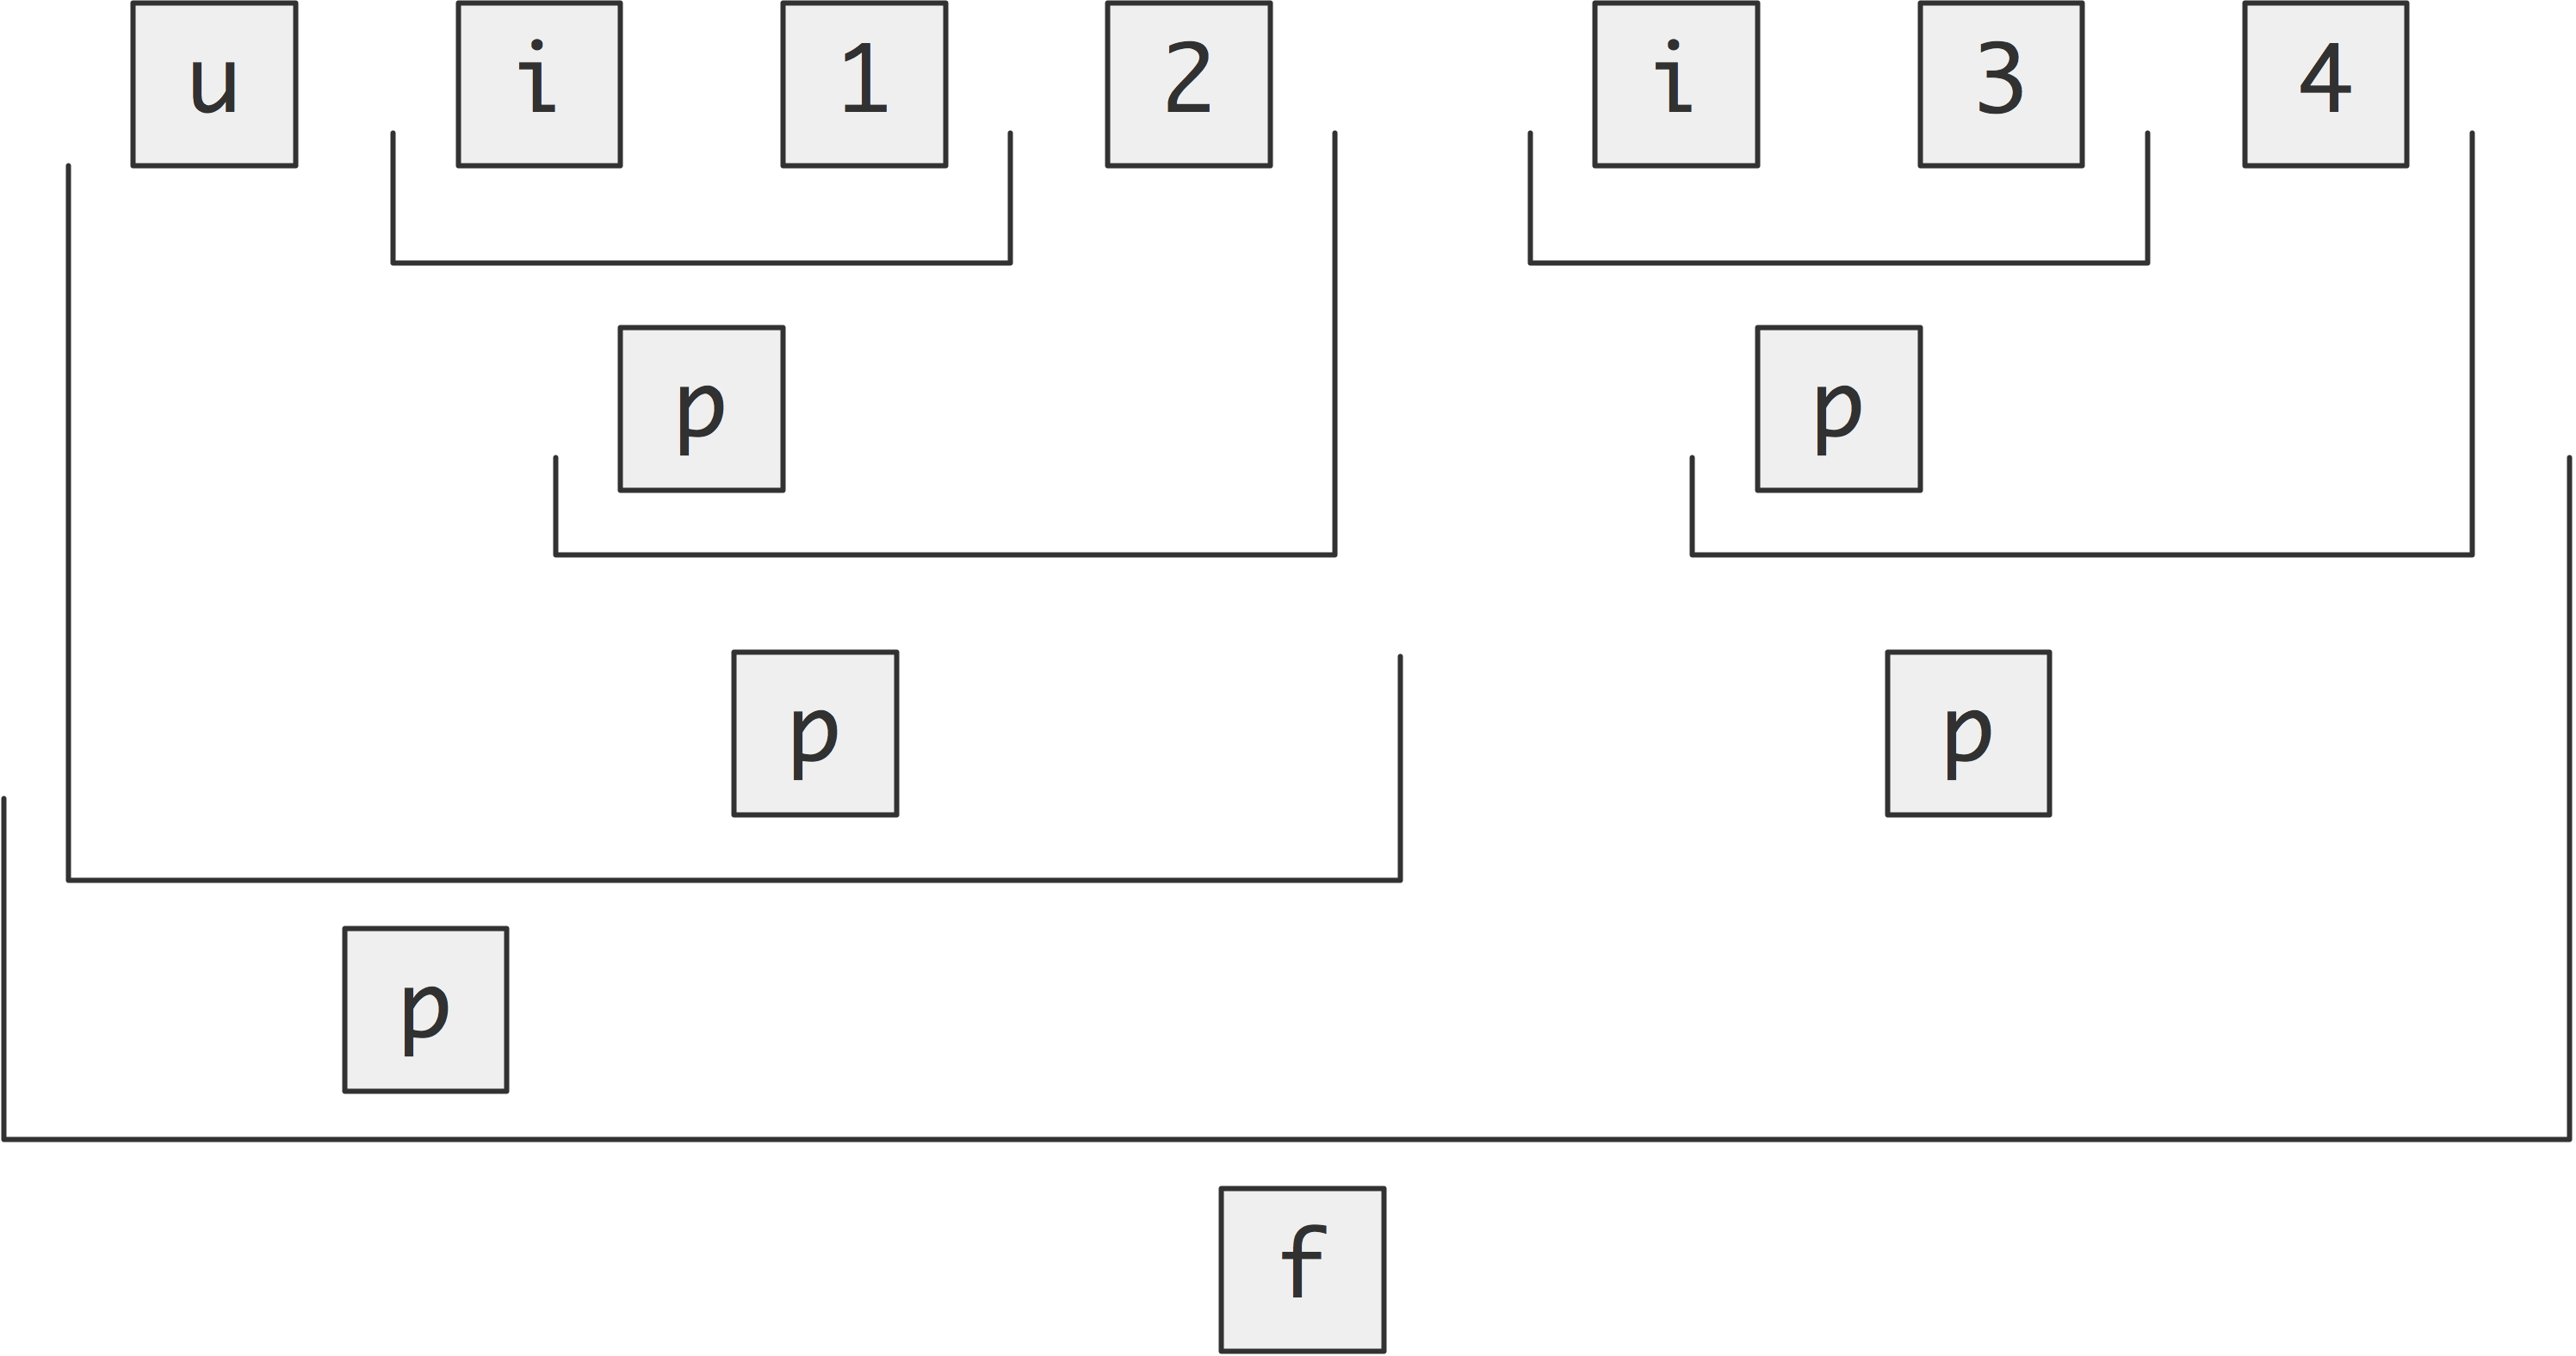
\includegraphics[scale=.1]{omp-reduct}
  \caption{Reduction of four items on two threads, taking into account
    initial values.}
  \label{fig:omp-reduct}  
\end{figure}
%
Figure~\ref{fig:omp-reduct} illustrates this, where \n{1,2,3,4} are
four data items, \n{i}~is the OpenMP initialization, and \n{u}~is the
user initialization; each \n{p}~stands for a partial reduction value.
The figure is based on execution using two threads.

\begin{exercise}
  Write a program to test the fact that the partial results
  are initialized to the unit of the reduction operator.
\end{exercise}

\Level 0 {User-defined reductions}
\index{omp!reduction!user-defined|(textbf}

With \emph{user-defined reductions}, the programmer specifies the
function that does the elementwise comparison.
This takes two steps.
\begin{enumerate}
\item You need a function of two arguments that returns the result of
  the comparison. You can do this yourself, but, especially with the
  C++ standard library, you can use functions such as \n{std::vector::insert}.
\item Specifying how this function operates on two variables
  \indexompshow{omp_out} and \indexompshow{omp_in}, corresponding to the
  partially reduced result and the new operand respectively. The new
  partial result should be left in \n{omp_out}.
\item Optionally, you can specify the value to which the reduction
  should be initialized.
\end{enumerate}

This is the syntax of the definition of the reduction, which can then
be used in multiple \indexclause{reduction} clauses.
\begin{lstlisting}
#pragma omp declare reduction 
    ( identifier : typelist : combiner )
    [initializer(initializer-expression)]
\end{lstlisting}
where:
\begin{description}
  \item[\texttt{identifier}] is a name; this can be overloaded for
    different types, and redefined in inner scopes.
  \item[\texttt{typelist}] is a list of types.
  \item[\texttt{combiner}] is an expression that updates the internal
    variable \indexompshow{omp_out} as function of itself and \indexompshow{omp_in}.
  \item[\texttt{initializer}] sets \indexompshow{omp_priv} to the
    identity of the reduction; this
    can be an expression or a brace initializer.
\end{description}

For instance, recreating the maximum reduction would look like this:
%
\cverbatimsnippet[examples/omp/c/ireduct.c]{ompmymax}

\begin{exercise}
  Write a reduction routine that operates on an array of nonnegative
  integers, finding the smallest nonzero one. If the array has size
  zero, or entirely consists of zeros, return~\n{-1}.
\end{exercise}

Support for
\emph{C++ iterators}\index{C++ iterators!in OMP reduction}
\begin{lstlisting}
#pragma omp declare reduction (merge : std::vector<int>
  : omp_out.insert(omp_out.end(), omp_in.begin(), omp_in.end())) 
\end{lstlisting}

\index{omp!reduction!user-defined|)}

\Level 0 {Reductions and floating-point math}

The mechanisms that OpenMP uses to make a reduction parallel go
against the strict rules for floating point expression evaluation in~C;
see~\HPSCref{sec:round-compile}. OpenMP ignores this issue: it is the
programmer's job to ensure proper rounding behaviour.

\index{omp!reduction|)}
